% homework/alg13p3/alg13p3.tex
% Algebra Track - Project 3 - Somebody Is 2.7 Kilometres Away.
%
% NOT a Year 7 packet. This is the TWO-SIDED, LANDSCAPE working sheet for the
% high-school Algebra Track project in content/freshman-math/P03_1/, printed
% from the site's Homework shelf. One sheet, one student.
%
%   FRONT  the three app readings, then the Hoi An map at exactly 1 cm = 250 m.
%          Almost the whole side is map, because the side is a drawing surface:
%          the 2.7 km arc alone has a 10.8 cm radius.
%   BACK   Q1-Q5, the privacy question, and the planning grid plus tear-off clue
%          card for the Early Years treasure hunt.
%
% THE SCALE IS LOad-BEARING AND MUST NOT BE "TIDIED". The map is included at
% exactly 25.6 cm wide, which makes it 1 cm = 250 m and 1 km = 4 cm, and the
% deck tells students to convert 2.7 km to a 10.8 cm radius on that basis. If
% anybody ever rescales the \includegraphics, the slides become wrong. The scale
% BAR drawn on the map is the fallback authority, and it is why it is there.
%
% The map file is not copied in beside this one - the \includegraphics reaches
% across to content/freshman-math/P03_1/images/hoi-an-map.png so that the sheet
% on the desk and the map on the projector cannot drift apart. Its licence is
% ODbL and the "Map data (c) OpenStreetMap contributors" credit is burned into
% the image itself, bottom right, which is exactly why it is burned in: this
% sheet leaves the building.
%
% The source is pure ASCII: every typographic character goes through a LaTeX
% command, so no editor or shell can mangle the encoding.
%
% Build:  pdflatex alg13p3.tex   (run twice)

\documentclass[12pt,a4paper]{article}

% -- Answer key switch -------------------------------------------------------
% There is no answer key PDF for this sheet - the marking guidance is in the
% lesson plan, and half the sheet has no single right answer. The switch is kept
% so the shared build script's teacher pass does not fail.
\newif\ifkey
\ifdefined\TEACHER\keytrue\else
  \keyfalse
\fi

% -- House style -------------------------------------------------------------
% homework/hw-style.tex
% Shared house style for every Year 7 homework packet. \input this from the
% packet file, right after \documentclass and the answer-key switch.
%
% Do not fork this file per packet. If a packet needs a different look, the
% question is whether every packet should have it.
%
% The choices here are deliberate and were arrived at by printing and looking:
%   * No solid dark banners. Every header is a light tint with a coloured spine
%     on the left, so colour reads clearly without flooding a school printer.
%   * No marks and no mark totals. These are practice, not exam papers.
%   * Lato at 12pt with open leading, plus mathastext so inline maths is Lato
%     too. Without mathastext every "-6 + 4" is Computer Modern serif and the
%     sheet looks half-typeset.
%   * Writing lines are spaced for Year 7 handwriting, not adult margin notes.
%
% Provides: \wlines \blank \tickbox \sep \qmk-free marks (none) \hwsection
% \qhead \expr, the workspace box, and the remember / wordhelp / activity /
% yourturn coloured boxes. Palette matches the lesson decks exactly.

% -- Packages ----------------------------------------------------------------
\usepackage[T1]{fontenc}
\usepackage[utf8]{inputenc}
\usepackage[default]{lato}
\usepackage[a4paper,top=1.7cm,bottom=1.7cm,left=2.0cm,right=2.0cm,headheight=15pt]{geometry}
\usepackage{amsmath,amssymb}
\usepackage{xcolor}
\usepackage[most]{tcolorbox}
\usepackage{enumitem}
\usepackage{tikz}
\usetikzlibrary{arrows.meta}
\usepackage{array}
\usepackage{tabularx}
\usepackage{fancyhdr}
\usepackage{multicol}
\usepackage{needspace}
\usepackage{graphicx}

% Make maths use Lato too. Without this, every "-6 + 4" on the page is set in
% Computer Modern serif and the sheet looks half-typeset. Must come last.
\usepackage[italic]{mathastext}

\linespread{1.06}\selectfont

% -- The Learner's Book palette (same hex values as the lesson decks) ---------
\definecolor{cbteal}{HTML}{0087A8}
\definecolor{cbpurple}{HTML}{5C2483}
\definecolor{cborange}{HTML}{C25E12}
\definecolor{cbgreen}{HTML}{4A8B23}
\definecolor{cbred}{HTML}{C8102E}
\definecolor{cbblue}{HTML}{1A5FA8}
\definecolor{rulegray}{HTML}{9AA5AD}

% -- Answer lines and blanks -------------------------------------------------
% \wlines{n} draws n ruled writing lines, spaced wide enough for Year 7
% handwriting rather than for an adult with a fine pen.
\makeatletter
\newcommand{\wlines}[1]{%
  \par\vspace{0.75em}%
  \@tempcnta=0\relax
  \@whilenum\@tempcnta<#1\do{%
    \hbox to \linewidth{\color{rulegray}\leaders\hrule height 0.5pt\hfill}%
    \vspace{1.5em}%
    \advance\@tempcnta by 1\relax}%
  \par\vspace{-0.8em}%
}
\makeatother

% \blank[width] is an inline gap to write a short answer in.
\newcommand{\blank}[1][2.6cm]{\underline{\hspace{#1}}}

% A boxed space for showing working.
\newtcolorbox{workspace}[1][3.4cm]{%
  colback=white, colframe=rulegray, boxrule=0.5pt, arc=5pt,
  height=#1, left=6pt, right=6pt, top=4pt, bottom=4pt,
  before skip=9pt, after skip=11pt}

% An empty tick box.
\newcommand{\tickbox}{\fbox{\rule{0pt}{1.15em}\rule{1.15em}{0pt}}}

% A middot separator.
\newcommand{\sep}{\,\textperiodcentered\,}

% -- Section and question headings -------------------------------------------
% Light tint plus a fat coloured spine on the left. No solid dark banner: the
% colour reads clearly but barely costs the printer anything.
% needspace stops a heading stranding alone at the foot of a page. Kept modest:
% too large and it pushes headings over, leaving a worse hole than it prevents.
\newcommand{\hwsection}[2][cbteal]{%
  \needspace{8\baselineskip}%
  \par\vspace{13pt}%
  \noindent
  \begin{tcolorbox}[enhanced, nobeforeafter, width=\textwidth,
      colback=#1!7, colframe=#1!7, arc=5pt,
      borderline west={5pt}{0pt}{#1},
      left=14pt, right=10pt, top=7pt, bottom=7pt]
    {\large\bfseries\color{#1}#2}
  \end{tcolorbox}%
  \par\vspace{9pt}}

% \qhead[colour]{A2}{Moving along the line} -- a question heading.
\newcommand{\qhead}[3][cbteal]{%
  \needspace{6\baselineskip}%
  \par\vspace{11pt}%
  \noindent{\large\bfseries\color{#1}#2}\quad{\large\bfseries #3}\par\vspace{4pt}}

% -- Coloured boxes ----------------------------------------------------------
% Shared look: rounded, light fill, coloured rule, coloured title text on a
% pale title strip rather than a dark one.
\tcbset{hwbox/.style={
  enhanced, breakable, arc=6pt, boxrule=1pt,
  left=11pt, right=11pt, top=8pt, bottom=8pt,
  fonttitle=\bfseries, attach boxed title to top left={xshift=12pt, yshift=-8pt},
  boxed title style={arc=4pt, boxrule=1pt, left=7pt, right=7pt, top=2pt, bottom=2pt},
  top=13pt}}

% Orange: things to remember. Matches the deck's "Write This Down".
\newtcolorbox{remember}[1][Remember from the lesson]{hwbox,
  colback=cborange!6, colframe=cborange, coltitle=cborange,
  colbacktitle=white, title={#1}}

% Blue: English help. The barrier in this class is the wording, not the maths.
\newtcolorbox{wordhelp}[1][Word help]{hwbox,
  colback=cbblue!6, colframe=cbblue, coltitle=cbblue,
  colbacktitle=white, title={#1}}

% Purple: an activity or instruction.
\newtcolorbox{activity}[1][How to do this homework]{hwbox,
  colback=cbpurple!6, colframe=cbpurple, coltitle=cbpurple,
  colbacktitle=white, title={#1}}

% Green: your turn / a friendly nudge.
\newtcolorbox{yourturn}[1][Your turn]{hwbox,
  colback=cbgreen!7, colframe=cbgreen, coltitle=cbgreen!75!black,
  colbacktitle=white, title={#1}}

% -- Shorthands --------------------------------------------------------------
\newcommand{\dC}{\,^{\circ}\mathrm{C}}          % use inside maths: $-8\dC$
\newcommand{\key}[1]{{\color{cborange}\textbf{#1}}}
\newcommand{\eng}[1]{{\color{cbblue}\textbf{#1}}}

\setlist[enumerate]{itemsep=8pt, topsep=5pt, leftmargin=*}
\setlist[itemize]{itemsep=4pt, topsep=4pt, leftmargin=*}
\renewcommand{\arraystretch}{1.45}

% -- An expression the student is asked to work from -------------------------
\newcommand{\expr}[1]{%
  \tcbox[on line, colback=cbgreen!10, colframe=cbgreen!55, boxrule=1pt, arc=4pt,
         left=9pt, right=9pt, top=4pt, bottom=4pt]{\large\bfseries $#1$}}

% -- Running head and foot ---------------------------------------------------
% The packet overrides \fancyhead[L] with its own title.
\pagestyle{fancy}
\fancyhf{}
\fancyhead[L]{\small\color{black!55}Year 7\sep Homework}
\fancyhead[R]{\small\color{black!55}Name: \blank[3.4cm]}
\fancyfoot[C]{\small\color{black!55}Page \thepage}
\renewcommand{\headrulewidth}{0pt}
\renewcommand{\headrule}{\vspace{2pt}\hbox to\headwidth{\color{cbteal!45}\leaders\hrule height 1.2pt\hfill}}



% Landscape, tight margins: both sides are working surfaces.
% includeheadfoot is load-bearing - without it geometry measures `top` to the
% top of the BODY and hangs the running head off the top of the sheet.
\geometry{landscape, top=1.0cm, bottom=0.8cm, left=1.3cm, right=1.3cm,
          includeheadfoot, headsep=7pt}

% Kept short: the full lesson title here ran straight into the scale note on the
% right and the two overprinted each other.
\fancyhead[L]{\small\color{black!55}Algebra Track\sep Project 3}
% The scale lives in the running head rather than in a banner on the back. As a
% banner it cost 1.5 cm at the top of page 2, which was exactly enough to push
% the two-column row onto a third page and leave page 2 holding nothing but the
% banner. Here it is on both sides, where it is wanted, and costs nothing.
\fancyhead[R]{\small\color{black!55}1 cm on the map = 250 m}
\fancyfoot[C]{\small\color{black!40}Page \thepage\ of 2}

% A reading chip: letter, place, distance.
\newcommand{\reading}[3]{%
  \begin{tcolorbox}[enhanced, nobeforeafter, width=8.1cm, colback=cborange!7,
      colframe=cborange!7, arc=5pt, borderline west={4pt}{0pt}{cborange},
      left=9pt, right=8pt, top=5pt, bottom=5pt]
    {\color{cborange}\bfseries #1}\quad #2\hfill{\bfseries\large #3}
  \end{tcolorbox}}

\begin{document}

% ===========================================================================
% FRONT - THE MAP
% ===========================================================================
\thispagestyle{fancy}

\noindent
\begin{tcolorbox}[enhanced, nobeforeafter, width=\textwidth,
                  colback=cbpurple!7, colframe=cbpurple!7, arc=6pt,
                  borderline west={6pt}{0pt}{cbpurple},
                  left=16pt, right=12pt, top=5pt, bottom=5pt]
  {\color{cbpurple}\bfseries PROJECT 3}\quad
  {\color{cbpurple}\large\bfseries Somebody Is 2.7 Kilometres Away}\quad
  {\color{black!60}\small Neary says: \textit{"We never share your location."}}\hfill
  {\color{black!70}\bfseries Name: \blank[4.2cm]}
\end{tcolorbox}

\vspace{3pt}

\noindent
\reading{A}{Japanese Bridge}{2.7 km}\hfill
\reading{B}{Tra Que Herb Village}{1.5 km}\hfill
\reading{C}{Cua Dai Beach}{2.3 km}

\vspace{3pt}

\noindent
\begin{tikzpicture}
  \node[anchor=south west, inner sep=0, draw=rulegray, line width=0.5pt] (map) at (0,0)
    {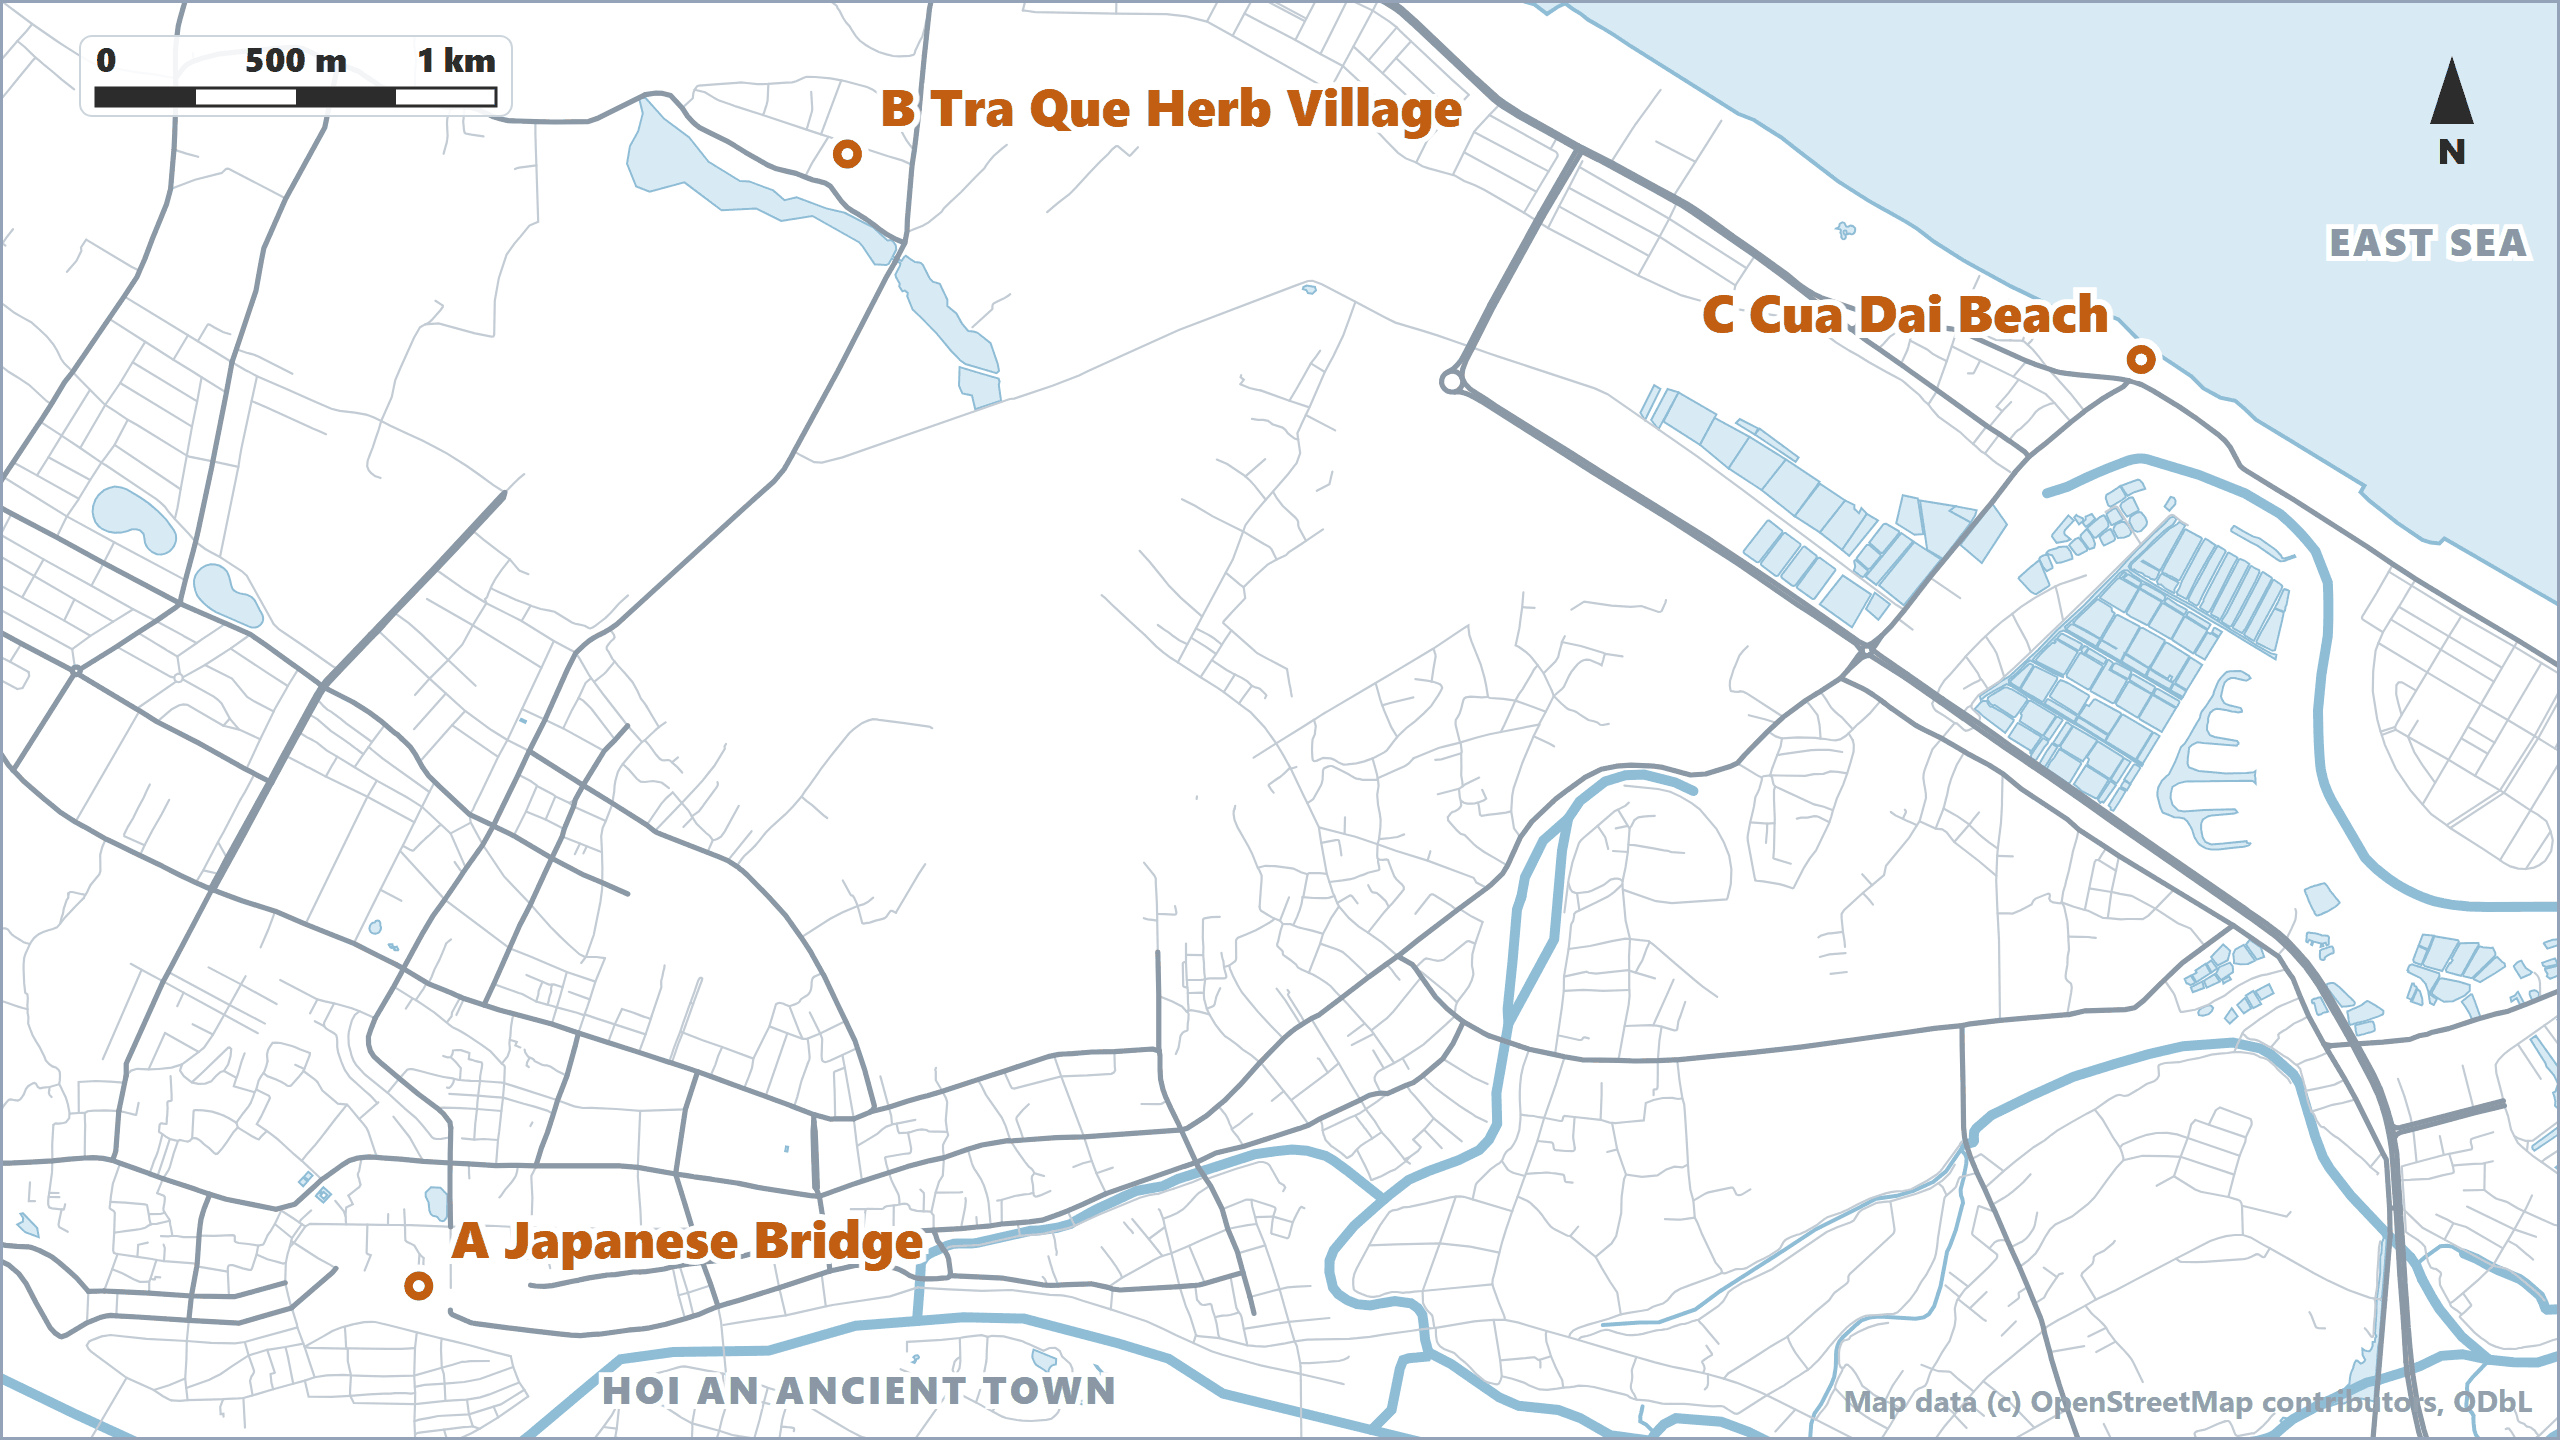
\includegraphics[width=25.6cm]{../../content/freshman-math/P03_1/images/hoi-an-map.png}};
\end{tikzpicture}

\newpage

% ===========================================================================
% BACK - THE WRITE-UP AND THE TREASURE GRID
% ===========================================================================
\noindent
\begin{minipage}[t]{13.1cm}
  \vspace{0pt}

  \qhead[cborange]{Q1}{Two answers before one}
  \vspace{-3pt}
  {\small Using only readings \textbf{A} and \textbf{B}, mark \emph{both} places the two
  arcs cross. Name them.}
  \vspace{2pt}

  {\small First crossing:} \blank[8.3cm]\\[7pt]
  {\small Second crossing:} \blank[8.0cm]

  \qhead[cborange]{Q2}{Where is he?}
  \vspace{-3pt}
  {\small Now bring in reading \textbf{C}. One crossing survives. Finish the sentence.}
  \vspace{4pt}

  {\small Mr Bowen is at} \blank[9.6cm]

  \qhead[cbgreen]{Q3}{How sure are you, in metres?}
  \vspace{-3pt}
  {\small Your three arcs will not meet at a point --- they bound a small patch.
  Measure it, then convert it.}
  \vspace{3pt}

  \begin{tabularx}{\dimexpr\linewidth-3\arrayrulewidth\relax}{|X|p{3.1cm}|p{3.1cm}|}
    \hline
    \rule[-0.35em]{0pt}{1.5em} & \textbf{across (mm)} & \textbf{in metres} \\
    \hline
    \rule[-0.5em]{0pt}{1.7em}widest way across the patch & & \\
    \hline
  \end{tabularx}
  \vspace{2pt}

  {\small Show the conversion:}
  \begin{workspace}[1.6cm]\end{workspace}

  % The bottom of this column was empty, and the hunt downstairs needs a thing
  % to physically hand over. A dashed border because it gets torn off.
  \vspace{4pt}
  {\small\bfseries\color{cbpurple}Tear this off and hand it to the Early Years team.}
  \vspace{3pt}

  \begin{tcolorbox}[enhanced, nobeforeafter, width=\linewidth, colback=white,
      boxrule=0pt, arc=4pt, borderline={1pt}{0pt}{cbpurple, dashed},
      left=10pt, right=10pt, top=7pt, bottom=7pt, fontupper=\small]
    {\color{cbpurple}\bfseries TREASURE CLUE CARD}\hfill Team: \blank[3.4cm]\\[6pt]
    From \textbf{P} (\blank[3.1cm]) it is \blank[1.7cm] m\\[4pt]
    From \textbf{Q} (\blank[3.1cm]) it is \blank[1.7cm] m\\[4pt]
    From \textbf{R} (\blank[3.1cm]) it is \blank[1.7cm] m
  \end{tcolorbox}
\end{minipage}%
\hfill
\begin{minipage}[t]{13.1cm}
  \vspace{0pt}

  \qhead[cbred]{Q4}{What this means for your phone}
  \vspace{-3pt}
  {\small An app shows only how far away you are, to the nearest 0.1 km. Why is
  that still worth being careful about? Name one thing you would check in its
  settings.}
  \vspace{-2pt}
  \wlines{4}

  \qhead[cbpurple]{Part 2}{The treasure hunt --- planning grid}
  \vspace{-3pt}
  {\small Three fixed points, \key{not in a straight line}. Describe each one well
  enough for a stranger to stand on it. Distances to the nearest 10 cm.}
  \vspace{3pt}

  \begin{tabularx}{\dimexpr\linewidth-4\arrayrulewidth\relax}{|p{1.0cm}|X|p{3.0cm}|}
    \hline
    \rule[-0.35em]{0pt}{1.5em}\textbf{} & \textbf{What it is, exactly} & \textbf{Distance (m)} \\
    \hline
    \rule[-0.5em]{0pt}{1.8em}\textbf{P} & & \\
    \hline
    \rule[-0.5em]{0pt}{1.8em}\textbf{Q} & & \\
    \hline
    \rule[-0.5em]{0pt}{1.8em}\textbf{R} & & \\
    \hline
  \end{tabularx}

  \qhead[cbteal]{Q5}{What actually happened}
  \vspace{-3pt}
  {\small Did your clues work first time? If they went to the wrong place first,
  \emph{which} wrong place --- and why would two distances allow it?}
  \vspace{-2pt}
  \wlines{3}
\end{minipage}

\end{document}
